\documentclass[10pt]{beamer}
\usetheme[progressstyle=movingCircCnt]{Feather}
  
% If you want to change the colors of the various elements in the theme, edit and uncomment the following lines
\definecolor{CardinalRed}{RGB}{140, 21, 21}
\definecolor{CoolGrey}{RGB}{77, 79, 83}
\definecolor{Black}{RGB}{46, 45, 41}
\definecolor{Sandstone}{RGB}{210, 194, 149}
\setbeamercolor{block title}{bg=Sandstone}

% Change the bar colors:
\setbeamercolor{Feather}{fg=Sandstone,bg=CardinalRed}

% Change the color of the structural elements:
\setbeamercolor{structure}{fg=CoolGrey}

% Change the frame title text color:
%\setbeamercolor{frametitle}{fg=Sandstone}

% Change the normal text color background:
\setbeamercolor{normal text}{fg=Black}

%-------------------------------------------------------
% INCLUDE PACKAGES
%-------------------------------------------------------

\usepackage[utf8]{inputenc}
\usepackage[english]{babel}
\usepackage[T1]{fontenc}
\usepackage[scaled=0.9]{helvet}
\usepackage{bibentry,graphicx,subcaption,amsfonts,amssymb,amsthm,amsmath,verbatim,multicol,tikz-cd,multirow,booktabs,hyperref}

\captionsetup[figure]{labelformat=empty}
\setbeamertemplate{section in toc}[ball unnumbered]

\usepackage{algorithm}
\usepackage{algorithmic}

\floatname{algorithm}{Procedure}
\renewcommand{\algorithmicrequire}{\textbf{Input:}}
\renewcommand{\algorithmicensure}{\textbf{Output:}}

\newcommand{\eg}{{\it e.g.}}
\newcommand{\ie}{{\it i.e.}}
\newcommand{\ones}{\mathbf 1}

\newtheorem{thm}{Theorem}[section]
\newtheorem{lem}[thm]{Lemma}
\theoremstyle{remark}
\newtheorem*{rmk}{Remark}
\theoremstyle{definition}
\newtheorem{dfn}{Definition}

%-------------------------------------------------------
% DEFFINING AND REDEFINING COMMANDS
%-------------------------------------------------------

% colored hyperlinks
\newcommand{\chref}[2]{
  \href{#1}{{\usebeamercolor[bg]{Feather}#2}}
}

%-------------------------------------------------------
% INFORMATION IN THE TITLE PAGE
%-------------------------------------------------------

\title[] % [] is optional - is placed on the bottom of the sidebar on every slide
{ % is placed on the title page

\includegraphics[width=0.5\textwidth]{figures/ipm_logo_en_black.png}
}

\subtitle[University Ph.D. Dissertation Defense]
{
      \Large\textbf{\textsc{Applications of convex optimization in metabolic network analysis}}
}

\author[Mojtaba Tefagh]
{
\large\textsl{Mojtaba Tefagh}
}

\institute[Stanford University]
{
      \normalsize\emph{Information Systems Laboratory, Electrical Engineering Department,
      Stanford University}
  
  %there must be an empty line above this line - otherwise some unwanted space is added between the university and the country (I do not know why;( )
}

\date{\today}

%-------------------------------------------------------
% THE BODY OF THE PRESENTATION
%-------------------------------------------------------

\begin{document}

%-------------------------------------------------------
% THE TITLEPAGE
%-------------------------------------------------------

{\1% % this is the name of the PDF file for the background
\begin{frame}[plain,noframenumbering] % the plain option removes the header from the title page, noframenumbering removes the numbering of this frame only
\vspace{10pt}
  \titlepage % call the title page information from above
\end{frame}}


%-------------------------------------------------------
\begin{frame}{Outline}{}
%-------------------------------------------------------
\noindent
\begin{minipage}[t]{.49\textwidth}
\raggedright
\tableofcontents
\end{minipage}
\hfill
\begin{minipage}[t]{.49\textwidth}
\raggedleft
  \begin{figure}[ht]
    \centering
    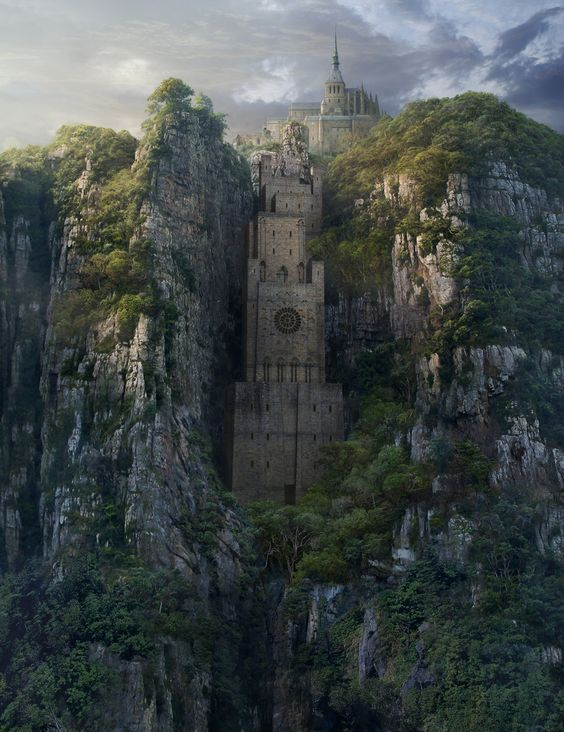
\includegraphics[width=\textwidth]{figures/3.png}
  \end{figure}
\end{minipage}
	
\end{frame}

%-------------------------------------------------------
\section{Motivation}
%-------------------------------------------------------
\begin{frame}{Motivation}{}
%-------------------------------------------------------
    
    \begin{figure}[ht]
    \centering
    \includegraphics[width=\textwidth]{figures/Genomics.jpg}
	\end{figure}
	
\end{frame}

%-------------------------------------------------------
\section{Introduction}
\subsection{Systems Biology}
%-------------------------------------------------------
\begin{frame}{Introduction}{Systems Biology}
%-------------------------------------------------------

\quad ``However, many things have a plurality of parts and are not merely a 
complete aggregate but instead some kind of a whole beyond its parts.'' 
\begin{flushright}
Aristotle, \emph{Metaphysics} \textbf{8.6}
\end{flushright}
    
    \begin{figure}[ht]
    \centering
    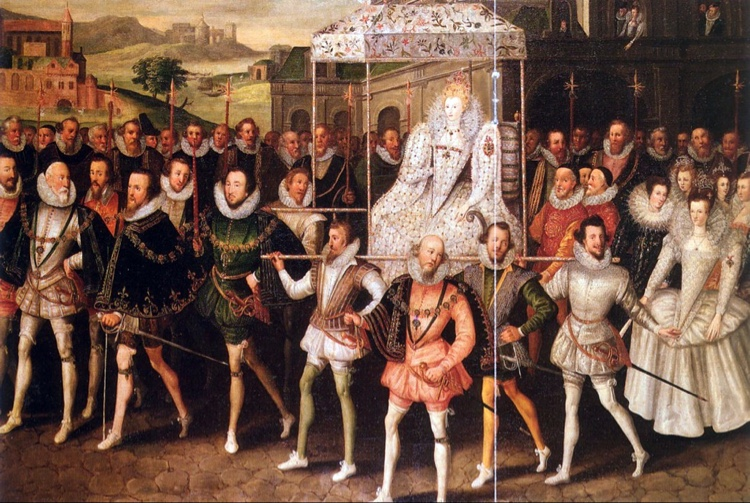
\includegraphics[width=0.8\textwidth]{figures/2.png}
    \caption{A metabolic network from KEGG pathway database}
	\end{figure}
	
\end{frame}

%-------------------------------------------------------
\subsection{COBRA}
\begin{frame}{Introduction}{COnstraint-Based Reconstruction and Analysis}
%-------------------------------------------------------
\noindent
\begin{minipage}[t]{.49\textwidth}
\raggedright
  \begin{itemize}
    \item<2-> Genome-scale metabolic network: $\mathcal{N} = (\mathcal{M}, \mathcal{R}, S, \mathcal{I})$
    \item<3-> Metabolites: $\mathcal{M} = \{M_i\}_{i=1}^m$
    \item<4-> Reactions: $\mathcal{R} = \{R_i\}_{i=1}^n$
    \item<5-> Stoichiometric matrix: $S$
    \item<6-> Irreversible reactions: $\mathcal{I} \subseteq \mathcal{R}$
    \item<7-> Flux distribution: $v\in\mathbf{R}^n$ 
	\item<8-> Mass balance condition: $Sv = 0$
    \item<9-> Thermodynamic directionality: $v_\mathcal{I} \geq 0$
    \item<10-> Steady-state flux cone: $\mathcal{C} = \{v \in \mathbf{R}^n \mid Sv=0,~ v_\mathcal{I} \geq 0\}$
    \item<11-> We call $R_i\in\mathcal{R}$ a blocked reaction if $v_i = 0,\quad\forall v\in\mathcal{C}$.
  \end{itemize}
\end{minipage}
\hfill
\begin{minipage}[t]{.49\textwidth}
\raggedleft
\begin{figure}[ht]
    \centering
    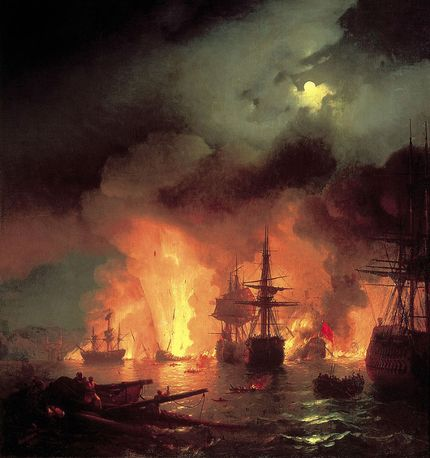
\includegraphics[width=\textwidth]{figures/4.jpg}
    \caption{Source: \cite{kim2012recent}}
  \end{figure}
\end{minipage}
\end{frame}

%-------------------------------------------------------
\section{Consistency Checking}
%-------------------------------------------------------
\begin{frame}{Consistency Checking}{The Naive Approach}
%-------------------------------------------------------

\begin{dfn}[\cite{schuster1994elementary}]
A metabolic network with no blocked reactions is called a flux
consistent metabolic network.
\end{dfn}\pause

By $n_i + 2 n_r$ LP's:\pause
  \begin{itemize}
    \item \textit{The forward direction:}
    \[
	\begin{array}{ll}
	\mbox{maximize}		& v_i \\
	\mbox{subject to}	& v \in \mathcal{C}\\
						& v_i \leq 1
	\end{array}
	\]\pause
    \item \textit{The reverse direction:} 
    \[
	\begin{array}{ll}
	\mbox{minimize}		& v_i \\
	\mbox{subject to}	& v \in \mathcal{C}\\
						& v_i \geq -1
	\end{array}
	\]
  \end{itemize}

\end{frame}
%-------------------------------------------------------
\begin{frame}{Consistency Checking}{\textsc{swiftcc}}
%-------------------------------------------------------
\noindent
\begin{minipage}[t]{.49\textwidth}
\raggedright
\begin{itemize}
  \item<1-> Identifying irreversible blocked reactions by,
  \[
	\begin{array}{ll}
	\mbox{maximize}		& \ones^T\min(v_\mathcal{I},\ones) \\
	\mbox{subject to}	& v \in \mathcal{C}.
	\end{array}
  \]\pause
  \item<2-> Equivalently,
  \[
	\begin{array}{ll}
	\mbox{maximize}		& \ones^T u \\
	\mbox{subject to}	& S v = 0\\
						& v_\mathcal{I} \geq u\\
						& \ones \geq u \geq 0.
  \end{array}
  \]
  \item<3-> Requires one LP. 
\end{itemize}
\end{minipage}
\hfill
\begin{minipage}[t]{.49\textwidth}
\raggedleft
\begin{itemize}
  \item<4-> Identifying reversible blocked reactions by,
  \[
	\begin{cases}
	Sx=0 \\
	e_i^T x = 1
    \end{cases}
  \]
  \item<5-> Requires one QR decomposition.  
\end{itemize}
\end{minipage}
  
\end{frame}

%-------------------------------------------------------
\begin{frame}{Consistency Checking}{Benchmark}
%-------------------------------------------------------
    \begin{figure}[ht]
    \centering
    \begin{subfigure}[b]{0.45\textwidth}
        \includegraphics[width=\textwidth]{figures/runtimecc.png}
    \end{subfigure}
    \qquad
    \begin{subfigure}[b]{0.45\textwidth}
        \includegraphics[width=\textwidth]{figures/runtimeccBox.png}
    \end{subfigure}
    \caption{\textsc{swiftcc} is more than $8\times$ faster than \textsc{fastcc} on average 
    over $29$ iterations of varying sizes for the Recon3D model.}
	\end{figure}

\end{frame}


%-------------------------------------------------------
\section{QFCA}
%-------------------------------------------------------
\subsection{Background}
\begin{frame}{QFCA}{Flux Coupling Analysis}
%-------------------------------------------------------
  \begin{block}{FCA~\cite{burgard2004flux}}
  Let $(R_i,R_j)$ be an arbitrary pair of unblocked reactions.
	\begin{description}
		\item<2->[Directional Coupling:] $R_i \longrightarrow R_j$ if 
        \[v_i \neq 0 \Rightarrow v_j \neq 0,\quad\forall v \in \mathcal{C}.\]
		\item<3->[Partial Coupling:] $R_i \longleftrightarrow R_j$ if
        \[v_i \neq 0 \Leftrightarrow v_j \neq 0,\quad\forall v \in \mathcal{C}.\]
		\item<4->[Full Coupling:] $R_i \Longleftrightarrow R_j$ if there exists a constant
        $c\neq0$ such that \[v_i = c v_j,\quad\forall v \in \mathcal{C}.\] 
	\end{description}
  \end{block}
\end{frame}


%-------------------------------------------------------
\begin{frame}{QFCA}{Feasibility-based Flux Coupling Analysis}
%-------------------------------------------------------

  \begin{block}{Problem}
  Given the stoichiometric matrix $S$ and the subset of irreversible reactions $\mathcal{I}$, 
  identify all the blocked reactions and the pairs of reactions which are directional, 
  partially, or fully coupled.
  \end{block}\pause
  
  \begin{block}{FFCA~\cite{david2011ffca}}
  By $n(n_i+2n_r)+2n_p$ LP's:
  \vspace{-20pt}
  \begin{multicols}{2}
  \[
  \begin{array}{ll}
  \mbox{maximize}	& v_i \\
  \mbox{subject to}	& v \in \mathcal{C}\\
		  			& v_j = 0\\
	  				& v_i \leq 1.
  \end{array}
  \]
  \[
	\begin{array}{ll}
	\mbox{maximize}		& v_i \\
	\mbox{subject to}	& v \in \mathcal{C}\\
						& v_j = 1.
	\end{array}
  \] 
  \break
  \vspace{-11pt}
  \[
  \begin{array}{ll}
  \mbox{minimize}	& v_i \\
  \mbox{subject to}	& v \in \mathcal{C}\\
		  			& v_j = 0\\
	  				& v_i \geq -1.
  \end{array}
  \]
  \[
	\begin{array}{ll}
	\mbox{minimize}		& v_i \\
	\mbox{subject to}	& v \in \mathcal{C}\\
						& v_j = 1.
	\end{array}
  \]

  \end{multicols}
  \end{block}
\end{frame}

%-------------------------------------------------------
\subsection{Flux Coupling Equations}
\begin{frame}{QFCA}{Directional Coupling Equation}
%-------------------------------------------------------
\noindent
\begin{minipage}[t]{.49\textwidth}
\raggedright
  \begin{itemize}
    \item<2-> For $R_{i_1}, R_{i_2}, \ldots, R_{i_l}\in\mathcal{I}$, there exists 
    $c_{i_1}, c_{i_2}, \ldots, c_{i_l} > 0$, such that
	\[
	v_j = c_{i_1}v_{i_1} + c_{i_2}v_{i_2} + \cdots + c_{i_l}v_{i_l}.
	\]
    \item<3-> There exists $c'_{i_{l+1}}\neq 0$,
    \[
    v_j = c'_{i_1}v_{i_1} + c'_{i_2}v_{i_2} + \cdots + c'_{i_{l+1}}v_{i_{l+1}}.
    \]
    \item<4-> 
    \[
	(1+\frac{1}{c})v_j = (c_{i_1}+\frac{c'_{i_1}}{c})v_{i_1} + (c_{i_2}+\frac{c'_{i_2}}{c})v_{i_2} 
	+ \cdots + (c_{i_l}+\frac{c'_{i_{l+1}}}{c})v_{i_l} + \frac{c'_{i_{l+1}}}{c}v_{i_{l+1}}
	\]
  \end{itemize}
\end{minipage}
\hfill
\begin{minipage}[t]{.49\textwidth}
\raggedleft
  \begin{figure}[ht]
	\centerline{\includegraphics[width=\textwidth]{figures/fig3.png}}
	\caption{For $t=2,3,4$, $R_t \longrightarrow R_1$ can be inferred from the DCE corresponding 
	to $M_1$.}
  \end{figure}
\end{minipage}

\end{frame}
%-------------------------------------------------------
\begin{frame}{QFCA}{Directional Coupling Equation}
%-------------------------------------------------------
\begin{thm}[\cite{Tefagh2018}]
		Suppose that $\mathcal{N} = (\mathcal{M}, \mathcal{R}, S, \mathcal{I})$ has no irreversible blocked 
		reactions. Let $R_j$ be an arbitrary unblocked reaction, and $\mathcal{D}_j\subseteq\mathcal{I}$ 
		denote the set of all the irreversible reactions which are directionally coupled to $R_j$ excluding 
		itself. Then, $\mathcal{D}_j\neq\emptyset$ if and only if there exists $c_d > 0$ for each 
		$R_d\in\mathcal{D}_j$, such that the following \emph{directional coupling equation} (DCE)
		\[
		v_j = \sum_{d:R_d\in\mathcal{D}_j}c_d v_d,
		\]
		holds for all $v\in\mathcal{C}$.
		Moreover, for any unblocked $R_i\notin\mathcal{I}$, we have $R_i \longrightarrow R_j$ 
		if and only if there exists an \emph{extended directional coupling equation} (EDCE)
		\[
		v_j = \sum_{d:R_d\in\mathcal{D}_j}c'_d v_d + c'_i v_i\qquad c'_i\neq 0,
		\]
		which holds for all $v\in\mathcal{C}$.
\end{thm}
\end{frame}

%-------------------------------------------------------
\begin{frame}{QFCA}{Flux Coupling Equations}
%-------------------------------------------------------

\begin{figure}[ht]
    \centering
    \begin{subfigure}[b]{0.45\textwidth}
        \includegraphics[width=\textwidth]{figures/fig1.png}
        \caption{the original metabolic network}
    \end{subfigure}
    \qquad
    \begin{subfigure}[b]{0.45\textwidth}
        \includegraphics[width=\textwidth]{figures/fig2.png}
        \caption{the transformed metabolic network}
    \end{subfigure}
    \begin{subfigure}[b]{0.45\textwidth}
        \includegraphics[width=\textwidth]{figures/original.png}
    \end{subfigure}
    \qquad
    \begin{subfigure}[b]{0.45\textwidth}
        \includegraphics[width=\textwidth]{figures/fig7.png}
    \end{subfigure}
    \caption{$R_2 \longrightarrow R_4$ can be inferred from the EDCEs corresponding to $M_1$ and $M_2$.}
\end{figure} 
\end{frame}

%-------------------------------------------------------
\begin{frame}{QFCA}{Flux Coupling Equations}
%-------------------------------------------------------

\begin{figure}[ht]
	\centerline{\includegraphics[scale=0.25]{figures/example.png}}
	\caption{$M_1$ and $M_1 + M_3$ provide EDCEs, $M_2$ and $M_2+M_3$ provide DCEs, and $M_3$ provides an FCE.}
\end{figure} 
\end{frame}

%-------------------------------------------------------
\subsection{Fictitious Metabolites}
\begin{frame}{QFCA}{Fictitious Metabolites}
%-------------------------------------------------------

	\begin{dfn}
	We call $\lambda\in\mathbf{R}^n$ a fictitious metabolite if there exists 
	$\nu \in \mathbf{R}^m$ such that $\lambda = S^T \nu$.
	\end{dfn}\pause
	
	\begin{thm}[]\label{range-thm}
	Suppose that in a given metabolic network specified by $S$ and $\mathcal{I}$, 
	there are no irreversible blocked reactions. Then for any $\lambda\in\mathbf{R}^n$, 
	$\lambda$ is a fictitious metabolite if and only if
	\[
	\lambda^Tv=0,\quad\forall v\in\mathcal{C}.
	\]
	\end{thm}\pause
	
	\begin{lem}\label{lemma}
	Suppose that in a given metabolic network specified by $S$ and $\mathcal{I}$, 
	there are no irreversible blocked reactions. Then for any $\lambda\in\mathbf{R}^n$, 
	\[
	\lambda^Tv=0,\quad\forall v\in\mathcal{C}\Leftrightarrow\lambda^Tu=0,\quad\forall u\in\mathrm{ker}(S).
	\]
	\end{lem}
\end{frame}

%-------------------------------------------------------
\begin{frame}{QFCA}{Fictitious Metabolites}
%-------------------------------------------------------
{\tiny
\[
\begin{split}
M = &4\times 13dpg[c] + 2\times 2pg[c] + 2\times 3pg[c]\\
	&+ 4.8756\times 6pgc[c] + 3.8756\times 6pgl[c] + 2\times actp[c]\\
	&- 2\times adp[c] - 4\times amp[c] + 2\times dhap[c]\\
	&- 1.8756\times e4p[c] + 2\times f6p[c] + 4\times fdp[c]\\
	&+ 2\times g3p[c] + 2\times g6p[c] + 2\times pep[c]\\
	&+ 2\times pi[c] + 1\times pi[e] - 5.7513 \times r5p[c]\\
	&+ 5.8756\times ru5p-D[c] - 1.8756\times s7p[c]\\
	&+ 5.8756\times xu5p-D[c]
\end{split}
\]
\pause
\begin{multicols}{2}
	\begin{itemize}
		\item 3-Phospho-D-glyceroyl-phosphate
		\item D-Glycerate-2-phosphate
		\item 3-Phospho-D-glycerate
		\item 6-Phospho-D-gluconate
		\item 6-phospho-D-glucono-1-5-lactone
		\item Acetyl-phosphate
		\item ADP
		\item AMP
		\item Dihydroxyacetone-phosphate
		\item D-Erythrose-4-phosphate
		\item D-Fructose-6-phosphate
		\item D-Fructose-1-6-bisphosphate
		\item Glyceraldehyde-3-phosphate
		\item D-Glucose-6-phosphate
		\item Phosphoenolpyruvate
		\item Phosphate (pi[c])
		\item Phosphate (pi[e])
		\item alpha-D-Ribose-5-phosphate
		\item D-Ribulose-5-phosphate
		\item Sedoheptulose-7-phosphate
		\item D-Xylulose-5-phosphate
	\end{itemize}
\end{multicols}
}
\end{frame}

%-------------------------------------------------------
\begin{frame}{QFCA}{Positive and Negative Certificates}
%-------------------------------------------------------

\begin{table}[!ht]\centering
\caption{a bird's eye view of QFCA}
{\footnotesize
\begin{tabular}{cccc}
\toprule
& positive certificates & negative certificates & $A$ \\
\midrule
$\mathcal{B}_R$ & \multirow{3}{*}{$
(S^{(A)})^T x = e_i^{(A)} 
$} & \multirow{3}{*}{$
\begin{array}{ll}
&S^{(A)}u=0 \\
&{e_i^{(A)}}^T u = 1
\end{array}
$} & $\emptyset$ \\
EDCE & & & $\mathcal{D}_j\cup\{R_j\}$ \\
FCE & & & $\{j\}$ \\
\addlinespace
$\mathcal{B}_I$ & \multirow{4}{*}{$
\begin{array}{ll}
\mbox{maximize}		& \ones^T\min(\lambda^{(A)},\ones) \\
\mbox{subject to}	& S^T \nu = \lambda \\
					& \lambda_i = 0,\quad i\notin\mathcal{I} \\
					& \lambda_i \geq 0,\quad i\in\mathcal{I}\setminus A
\end{array}
$} & \multirow{3}{*}{$
\begin{array}{ll}
\mbox{maximize}		& \ones^T\min(v_\mathcal{I},\ones) \\
\mbox{subject to}	& v \in \mathcal{C}\\
					& v_A = 0
\end{array}
$} & $\emptyset$ \\
DCE & & & $\{j\}$ \\
\addlinespace
\addlinespace
\addlinespace
\addlinespace
\addlinespace
\bottomrule
\end{tabular}
}
\end{table}\pause
  
  \begin{itemize}
	\item Certificates as potential differences\pause
    \item Certificates as fictitious metabolites\pause
    \item Certificates as generalizations of fully coupling constants
    \[
	v_1=-\frac{\lambda_2}{\lambda_1}v_2-\frac{\lambda_3}{\lambda_1}v_3-\cdots-\frac{\lambda_l}{\lambda_1}v_l
	\]
  \end{itemize}
\end{frame}

%-------------------------------------------------------
\subsection{Implementation}
\begin{frame}{QFCA}{Final Algorithm}
%-------------------------------------------------------


\begin{block}{QFCA}
\begin{algorithmic} \label{pseudocode}
\REQUIRE $\mathcal{M}, \mathcal{R}, S, \mathcal{I}$
\ENSURE $A, b$\pause
\STATE identifying and removing the blocked reactions from the metabolic network \pause
\STATE aggregating all the isozymes and removing the newly blocked reactions \pause
\STATE identifying the fully coupled pairs of reactions and merging each pair \pause
\STATE computing the set of fully reversible reactions and reversibility type pruning \pause
\STATE finding the directional and partial coupling relations by positive certificates 
\end{algorithmic}
\end{block}

\end{frame}

%-------------------------------------------------------
\begin{frame}{QFCA}{Benchmark}
%-------------------------------------------------------
\begin{figure}[ht]
    \centering
    \begin{subfigure}[b]{0.45\textwidth}
        \includegraphics[width=\textwidth]{figures/yeast.png}
        \caption{YEASTNET v3.0 with 2292 reversible and 49 irreversible reactions}
    \end{subfigure}
    \qquad
    \begin{subfigure}[b]{0.45\textwidth}
        \includegraphics[width=\textwidth]{figures/Recon3D.png}
        \caption{Recon3D with 5238 reversible and 5362 irreversible reactions}
    \end{subfigure}
    \caption{QFCA average runtime is 7\% and 68\%
    of F2C2 average runtime, respectively.}\label{fig:runtime}
\end{figure}

\end{frame}

%-------------------------------------------------------
\subsection{Applications}
\begin{frame}{QFCA}{Applications}
%-------------------------------------------------------
	\begin{itemize}
		\item A quantitative approach to FCA
		\[
		v_j \geq c v_i
		\]\pause
		Equivalently the optimal value of the following LP is zero.
		\[
		\begin{array}{ll}
			\mbox{minimize}		& v_j - c v_i \\
			\mbox{subject to}	& v \in \mathcal{C}
		\end{array}
		\]\pause
		Deriving the dual,
		\[
		\begin{array}{ll}
			\mbox{maximize}		& 0 \\
			\mbox{subject to}	& S^T \nu + e_j - c e_i = \lambda \\
								& \lambda_i = 0,\quad i\notin\mathcal{I} \\
								& \lambda_i \geq 0,\quad i\in\mathcal{I}
		\end{array}
		\]\pause
		As a result,
		\[
		(1-\lambda^\star_j)v_j = (c+\lambda^\star_i)v_i + \sum_{d\neq i,j} \lambda^\star_d v_d,
		\]\pause
		\item Sensitivity analysis\pause 
		\item The metabolic gap-filling problem
	\end{itemize}
\end{frame}

%-------------------------------------------------------
\section{Metabolic Network Reductions}
\begin{frame}{Metabolic Network Reductions}{A Toy example}
%-------------------------------------------------------
\noindent
\begin{minipage}[t]{.49\textwidth}
\raggedright
\[
\mathcal{N} = (\mathcal{M}, \mathcal{R}, S, \mathcal{I})
\] 
\[
\mathcal{M}=\{M_1, M_2, M_3\}
\]
\[
\mathcal{R}=\{R_1,R_2,R_3,R_4,R_5\}
\] 
\[
\mathcal{I}=\mathcal{R}
\]
\[
S = \left[
\begin{array}{ccccc}
+1 & -1 & 0 & +2 & 0\\
0 & +1 & -1 & 0 & 0\\
0 & 0 & 0 & +1 & -1
\end{array}
\right]
\]
\end{minipage}
\hfill
\begin{minipage}[t]{.49\textwidth}
\raggedleft
\begin{figure}[ht]
    \centering
    \includegraphics[width=\textwidth]{figures/Fig1.eps}
    \caption{the original metabolic network}
\end{figure}
\end{minipage}\pause
\[
v = \left[
\begin{array}{c}
v_1\\
v_2\\
v_3\\
v_4\\
v_5
\end{array}
\right] = \left[
\begin{array}{c}
v_1\\
v_3\\
v_3\\
v_4\\
v_5
\end{array}
\right] = \left[
\begin{array}{cccc}
+1 & 0 & 0 & 0\\
0 & +1 & 0 & 0\\
0 & +1 & 0 & 0\\
0 & 0 & +1 & 0\\
0 & 0 & 0 & +1
\end{array}
\right]\left[
\begin{array}{c}
v_1\\
v_3\\
v_4\\
v_5
\end{array}
\right].
\]
\end{frame}


%-------------------------------------------------------
\begin{frame}{Metabolic Network Reductions}{A Toy example}
%-------------------------------------------------------
\noindent
\begin{minipage}[t]{.49\textwidth}
\raggedright
\[
\tilde{S} = \left[
\begin{array}{cccc}
+1 & -1 & +2 & 0\\
0 & 0 & +1 & -1
\end{array}
\right]
\]
\[
\begin{array}{l}
\tilde{R}_1 \xrightarrow{r_1} \{R_1\} \\
\tilde{R}_3 \xrightarrow{r_1} \{R_2, R_3\} \\
\tilde{R}_4 \xrightarrow{r_1} \{R_4\} \\
\tilde{R}_5 \xrightarrow{r_1} \{R_5\}
\end{array}
\]
\end{minipage}
\hfill
\begin{minipage}[t]{.49\textwidth}
\raggedleft
\begin{figure}[ht]%figure2
    \centering
    \includegraphics[width=\textwidth]{figures/Fig2.eps}
    \caption{the reduced metabolic network}
\end{figure}
\end{minipage}\pause
\[
Sv = S \left[
\begin{array}{cccc}
+1 & 0 & 0 & 0\\
0 & +1 & 0 & 0\\
0 & +1 & 0 & 0\\
0 & 0 & +1 & 0\\
0 & 0 & 0 & +1
\end{array}
\right]\left[
\begin{array}{c}
v_1\\
v_3\\
v_4\\
v_5
\end{array}
\right] = \left[
\begin{array}{cccc}
+1 & -1 & +2 & 0\\
0 & 0 & 0 & 0\\
0 & 0 & +1 & -1
\end{array}
\right]\left[
\begin{array}{c}
v_1\\
v_3\\
v_4\\
v_5
\end{array}
\right]
\]
\end{frame}

%-------------------------------------------------------
\begin{frame}{Metabolic Network Reductions}{A Toy example}
%-------------------------------------------------------
\noindent
\begin{minipage}[t]{.49\textwidth}
\raggedright
\[
\tilde{S} = \left[
\begin{array}{cccc}
+1 & -1 & +2 & 0\\
0 & 0 & +1 & -1
\end{array}
\right]
\]
\[
\begin{array}{l}
\tilde{R}_1 \xrightarrow{r_2} \{R_1, R_2\} \\
\tilde{R}_3 \xrightarrow{r_2} \{R_3\} \\
\tilde{R}_4 \xrightarrow{r_2} \{R_2, R_4\} \\
\tilde{R}_5 \xrightarrow{r_2} \{R_5\},
\end{array}
\]
\end{minipage}
\hfill
\begin{minipage}[t]{.49\textwidth}
\raggedleft
\begin{figure}[ht]%figure3
    \centering
    \includegraphics[width=\textwidth]{figures/Fig3.eps}
    \caption{a DCE-induced reduction}
\end{figure}
\end{minipage}\pause
\[
v = \left[
\begin{array}{c}
v_1\\
v_2\\
v_3\\
v_4\\
v_5
\end{array}
\right] = \left[
\begin{array}{c}
v_1\\
v_1 + 2v_4\\
v_3\\
v_4\\
v_5
\end{array}
\right] =
\left[
\begin{array}{cccc}
+1 & 0 & 0 & 0\\
+1 & 0 & +2 & 0\\
0 & +1 & 0 & 0\\
0 & 0 & +1 & 0\\
0 & 0 & 0 & +1
\end{array}
\right]\left[
\begin{array}{c}
v_1\\
v_3\\
v_4\\
v_5
\end{array}
\right] 
\]
\end{frame}

%-------------------------------------------------------
\begin{frame}{Metabolic Network Reductions}{QFCA Reductions}
%-------------------------------------------------------
\noindent
\begin{minipage}[t]{.49\textwidth}
\raggedright
	\begin{itemize}
		\item<1-> First, we eliminate all the blocked reactions.
		\item<2-> Second, we merge all the fully coupled reactions.
		\item<3-> Third, we remove the eligible reactions by the DCE-induced reductions.
	\end{itemize}
	\pause
	\pause
	\pause
	\begin{block}{}
	\[
	\mathcal{N}\xleftarrow{\phi_1,r_1}\tilde{\mathcal{N}}_1\xleftarrow{\phi_2,r_2}\cdots
	\xleftarrow{\phi_{n-\tilde{n}},r_{n-\tilde{n}}}\tilde{\mathcal{N}}_{n-\tilde{n}}
	\]
	\[
	\tilde{S} = SPA
	\]
	\[
	\phi^{n-\tilde{n}}(\tilde{v})=PA\tilde{v}
	\]
	\end{block}
\end{minipage}
\hfill
\begin{minipage}[t]{.49\textwidth}
\raggedleft
\begin{figure}[ht]%figure3
    \centering
    \includegraphics[width=\textwidth]{figures/matrix.png}
\end{figure}
\end{minipage}

\end{frame}

%-------------------------------------------------------
\begin{frame}{Metabolic Network Reductions}{Canonical Reductions}
%-------------------------------------------------------
We say that the metabolic network 
$\tilde{\mathcal{N}}=(\tilde{\mathcal{M}}, \tilde{\mathcal{R}}, \tilde{S}, \tilde{\mathcal{I}})$ 
is a reduction of $\mathcal{N}=(\mathcal{M}, \mathcal{R}, S, \mathcal{I})$ if 
\begin{enumerate}
	\item<2-> there exists a surjection $\phi:\tilde{\mathcal{C}}\rightarrow \mathcal{C}$,
	\item<3-> there exists a reduction map $r:\tilde{\mathcal{R}}\rightarrow\mathcal{P}(\mathcal{R})$ such 
	that 
	\[
	r(\tilde{R}_i) \nsubseteq \bigcup_{k\neq i}r(\tilde{R}_k)\quad\forall\tilde{R}_i\in\tilde{\mathcal{R}},
	\]
	\item<4-> and the following diagram commutes
	\begin{figure}[ht]
    \centering
    \includegraphics[width=0.2\textwidth]{figures/diagram.png}
	\end{figure}
	where $\tilde{r}:\mathcal{P}(\tilde{\mathcal{R}})\rightarrow\mathcal{P}(\mathcal{R})$ is defined by 
	\[
	\tilde{r}(\{\tilde{R}_i\}_{i\in I}) = \bigcup_{i\in I} r(\tilde{R}_i).
	\]
\end{enumerate}
\end{frame}

%-------------------------------------------------------
\begin{frame}{Metabolic Network Reductions}{Canonical Reductions}
%-------------------------------------------------------
$\phi_1\circ\phi_2:\tilde{\mathcal{C}}_2 \rightarrow \mathcal{C}$ is a surjection 
	because the composition of surjective functions is surjective, 
	
\pause

$\tilde{r}_1\circ r_2:\tilde{\mathcal{R}}_2\rightarrow\mathcal{P}(\mathcal{R})$ is 
	a legitimate reduction map because for any $\tilde{R}_i\in\tilde{\mathcal{R}}_2$ we have  
	\[
	\exists \tilde{R}_j\in r_2(\tilde{R}_i)\setminus\bigcup_{k\neq i}r_2(\tilde{R}_k) \Rightarrow 
	\exists R_t\in r_1(\tilde{R}_j)\setminus\bigcup_{k\neq j}r_1(\tilde{R}_k) \Rightarrow 
	R_t\in\tilde{r}_1\circ r_2(\tilde{R}_i)\setminus\bigcup_{k\neq i}\tilde{r}_1\circ r_2(\tilde{R}_k),
	\]
	
\pause

and the following diagram commutes
	\begin{figure}[ht]
    \centering
    \includegraphics[width=0.2\textwidth]{figures/diagram2.png}
	\end{figure}
	because for any $\tilde{v}\in\tilde{\mathcal{C}}_2$
	\[
	\mathrm{supp}(\phi_1\circ\phi_2(\tilde{v}))=\tilde{r}_1(\mathrm{supp}(\phi_2(\tilde{v})))
	=\tilde{r}_1\circ\tilde{r}_2(\mathrm{supp}(\tilde{v})).
	\]
\end{frame}

%-------------------------------------------------------
\begin{frame}{Metabolic Network Reductions}{Canonical reductions preserve EM's}
%-------------------------------------------------------

\begin{dfn}[\cite{schuster1994elementary}]
We call a nonzero feasible flux distribution $0\neq v \in \mathcal{C}$ an \emph{elementary mode} (EM), 
if its support is minimal, or equivalently, if there does not exist any other nonzero feasible flux 
distribution $0\neq u\in\mathcal{C}$ such that $\mathrm{supp}(u) \subset \mathrm{supp}(v)$. 
\end{dfn}

\pause

\begin{block}{\emph{Minimal conserved pool identification} (MCPI)}
Replace FCA by \emph{Metabolite concentration coupling analysis} (MCCA) and everything works!
\end{block}

\end{frame}

%-------------------------------------------------------
\begin{frame}{Metabolic Network Reductions}{Canonical reductions are minimal}
%-------------------------------------------------------

\begin{thm}[The reduction theorem]
Suppose that $\tilde{\mathcal{N}} = (\tilde{\mathcal{M}}, \tilde{\mathcal{R}}, \tilde{S}, 
\tilde{\mathcal{I}})$ is a metabolic network reduction of $\mathcal{N}=(\mathcal{M}, \mathcal{R}, 
S, \mathcal{I})$ by the surjection $\phi:\tilde{\mathcal{C}}\rightarrow \mathcal{C}$ 
and the reduction map $r:\tilde{\mathcal{R}}\rightarrow\mathcal{P}(\mathcal{R})$. 
For each $\tilde{R}_i,\tilde{R}_j\in\tilde{\mathcal{R}}$ such that $\tilde{R}_i \longrightarrow 
\tilde{R}_j$, any reaction in $r(\tilde{R}_i)\setminus \bigcup_{k\neq i}r(\tilde{R}_k)$ is 
directionally coupled to any reaction in $r(\tilde{R}_j)$. Conversely, if there exists a 
reaction in $r(\tilde{R}_i)$ which is directionally coupled to some reaction in $r(\tilde{R}_j)
\setminus\bigcup_{k\neq j}r(\tilde{R}_k)$, then $\tilde{R}_i \longrightarrow \tilde{R}_j$.
\end{thm}

\pause

\begin{rmk}
By setting $i=j$ in the reduction theorem, any reaction in $r(\tilde{R}_i)\setminus \bigcup_{k\neq i}r(\tilde{R}_k)$ 
is directionally coupled to any reaction in $r(\tilde{R}_i)$. 
\end{rmk}

\end{frame}

%-------------------------------------------------------
\begin{frame}{Metabolic Network Reductions}{Benchmark}
%-------------------------------------------------------
\begin{figure}[ht]
    \centering
    \begin{subfigure}[b]{0.45\textwidth}
        \includegraphics[width=\textwidth]{figures/LP.png}
    \end{subfigure}
    \qquad
    \begin{subfigure}[b]{0.45\textwidth}
        \includegraphics[width=\textwidth]{figures/runtime.png}
    \end{subfigure}
    \caption{\textsc{swiftcore} runs more than $3\times$ faster on the reduced BiGG universal model}
    \label{fig:BiGG}
\end{figure}
\[m=13249, n=24311, nnz(S) = 95774\]
\[\tilde{m}=1278, \tilde{n}=10255, nnz(\tilde{S}) = 56457\]
\end{frame}

%-------------------------------------------------------
\begin{frame}{Metabolic Network Reductions}{Biological Intuition}
%-------------------------------------------------------
The DCE reduced reactions are...\pause
\begin{itemize}
	\item<2-> essential reactions
	\item<3-> exchange reactions
	\item<4-> of older evolutionary age 
	\item<5-> evolutionary more conserved 
	\item<6-> essential in a wide range of conditions
	\item<7-> their associated genes are more expressed
	\item<8-> the reactions that produce biomass metabolites uniquely
	\item<9-> the reactions enriching the vital metabolic processes of the cell
\end{itemize}

\begin{block}{}
Essential reactions are the symmetric counterpart of the blocked reactions.
\end{block}
\end{frame}

%-------------------------------------------------------
\section{Conclusions}
\begin{frame}{Conclusions}{}
%-------------------------------------------------------
  \begin{multicols}{2}
	\begin{itemize}
		\item<1-> QFCA
		\begin{itemize}
			\item<2-> Flux coupling equations
			\item<3-> Fictitious metabolites
			\item<4-> Better worst-case complexity
			\item<5-> Faster in practice
			\item<6-> Biologically interpretable 
			\item<7-> Providing lower bounds
			\item<8-> Robust to missing reactions
			\item<9-> Metabolic gap-filling problem
		\end{itemize}
		\item<10-> Metabolic Network Reduction 
		\begin{itemize}
			\item<11-> Decreasing the size
			\item<12-> Preserving sparsity
			\item<13-> Context-free reductions
			\item<14-> Preserving EM's 
			\item<15-> The first axiomatic framework
			\item<16-> Provable optimal efficiency 
			\item<17-> Speed up analysis in practice 
			\item<18-> Biologically interpretable
		\end{itemize}
	\end{itemize}
  \end{multicols}	
\end{frame}

%-------------------------------------------------------
\section{Further Topics}
\begin{frame}{Further Topics}{}
%-------------------------------------------------------

	\begin{itemize}
		\item<1-> Closure of a metabolic network
		\item<2-> \textsc{swiftcc++}
		\item<3-> \textsc{swiftcore}
		\item<4-> \textsc{swiftGapFill}
		\item<5-> \textsc{sparseQFCA}
		\item<6-> Inhibition analysis
		\item<7-> Biological fidelity
	\end{itemize}
	
\end{frame}

\iffalse

%-------------------------------------------------------
\section{Publications}
\begin{frame}{Publications}{}
%-------------------------------------------------------

	\begin{itemize}
		\item<1-> \textbf{Tefagh, M.} and Boyd, S. P. (2018) ``Quantitative flux coupling analysis." \emph{Journal of Mathematical Biology}.
		\item<2-> \textbf{Tefagh, M.} and Boyd, S. P. (2019) ``Metabolic network reductions." \emph{In review}.
		\item<3-> \textbf{Tefagh, M.} and Boyd, S. P. (2019) ``\textsc{swiftcore}: a tool for the context-specific reconstruction of genome-scale metabolic networks." \emph{In review}.
		\item<4-> \textbf{Tefagh, M.} and Boyd, S. P. (2019) ``Sparse quantitative flux coupling analysis." \emph{In review}.
	\end{itemize}

\end{frame}

%-------------------------------------------------------
\section{Acknowledgments}
\begin{frame}{Acknowledgments}{}
%-------------------------------------------------------

	\begin{itemize}
		\item<1-> Advisor: Prof. Stephen Boyd
		\item<2-> Dissertation committee: Prof. David Tse and Prof. Yinyu Ye
		\item<3-> Qualifying exam committee: Prof. Markus Covert and Prof. Aaron Sidford
		\item<4-> My family: Mother, father, brother, and sister.
		\item<5-> And all of my friends!
	\end{itemize}

\end{frame}

\fi

{\1
\begin{frame}[plain,noframenumbering]
  \finalpage{\huge \emph{Thank You!}}
\end{frame}}

{\1
\begin{frame}[plain,noframenumbering]
  \finalpage{\huge \emph{Any Questions?}}
\end{frame}}

%-------------------------------------------------------
\begin{frame}[plain,noframenumbering]
%-------------------------------------------------------

	\footnotesize
    \bibliographystyle{apalike}
	\bibliography{refs}

\end{frame}

\end{document}